\documentclass[a4paper]{article}
\usepackage[margin=1in]{geometry}
\usepackage[english]{babel}
\usepackage[utf8]{inputenc}
\usepackage{amsmath,graphicx,tikz,circuitikz,pgfplots,filecontents,pgfplotstable,booktabs}

\pgfplotsset{compat=1.8}
\usetikzlibrary{decorations.pathmorphing}

\usepackage[justification=centering]{caption}
\usetikzlibrary{arrows,fit,patterns}

\usetikzlibrary{matrix}


\title{Test Document for \LaTeX \ Figures}

\author{Joshua Gruenstein and Michael Truell}

\date{\today}

\begin{document}
	\maketitle

	\section{Figures}
	\centering

	\begin{figure}[ht]
		\centering
		\input{Kinematics.tex}
		\caption{Differential Drive Kinematics}
	\end{figure}

	\begin{figure}[ht]
		\centering
		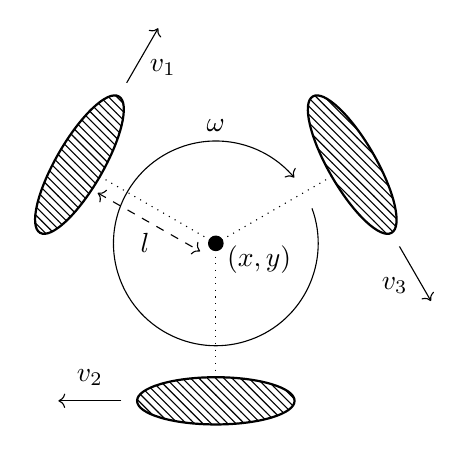
\begin{tikzpicture}
			\node[circle,fill,inner sep=-2pt] at (0,0){};
			\draw[->,rotate=20] (1.3,0) arc (0:-340:1.3cm);
			\draw[<->, dashed] (-1.5,0.64) -- (-0.2,-0.1);

			\node at (0.55,-0.2) {${(x,y)}$};
			\node at (0,1.5) {$\omega$};
			\node at (-0.9,0) {$l$};

			\foreach \r [count=\i] in {60,180,300} {
				\begin{scope}[rotate=\r]
					\draw[pattern=north west lines,thick](0,2) ellipse (1cm and 0.3cm);
					\draw[dotted] (0,0) -- (0,1.7);
					\draw[->] (1.2,2) -- (2,2);
					\node at (1.6,1.7) {$v_{\i}$};
				\end{scope}
			};
		\end{tikzpicture}
		\caption{Kiwi Drive Kinematics}
	\end{figure}


\end{document}

\end{document}
